\documentclass[../main.tex]{subfiles}
\graphicspath{{resources/}{resources/irodalom_res/}}
 
\begin{document}

\section{Okos LED-rendszerek felkutatása, forgalomban lévő eszközök áttekintése}
    Az evolúció során az emberi szem úgy fejlődött ki, hogy nappali fényhez - világoshoz - gyorsan alkalmazkodik és éles képet alkot. Sötéthez, szürkülethez csak lassan képes alkalmazkodni és akkor sem éles az a kép amit látunk. A fejlődő világunkban nélkülözhetetlenné vált a világítás, hogy napnyugta után sem álljon meg az élet és tovább tudjuk folytatni tevékenységeinket. //TODO - befejezni - egész kerek - kép kell nem?
    \begin{figure}[h!] %https://pixabay.com/en/city-night-lights-cityscape-urban-1967190/
        \centering
            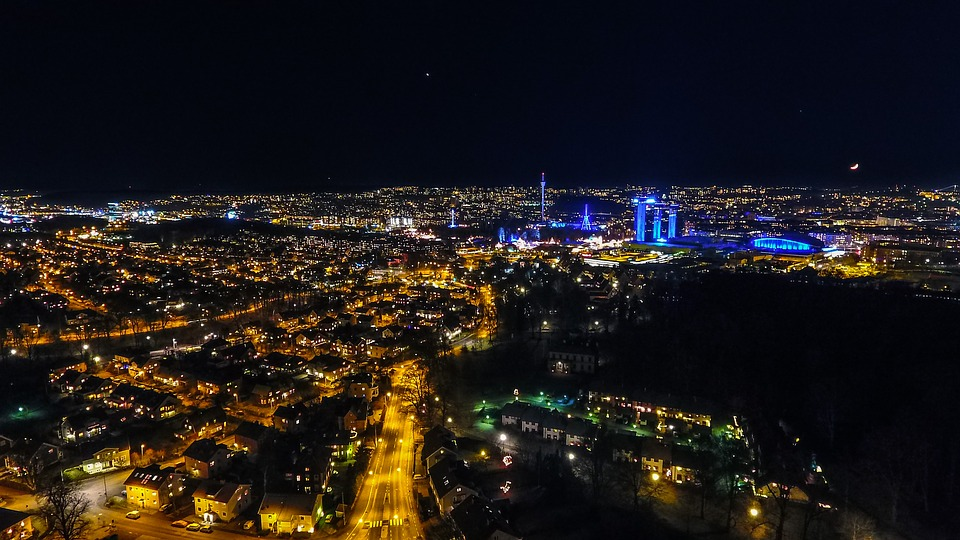
\includegraphics[height=7cm]{irodalom_res/night_life.jpg}
        \caption{Éjszakai város látképe} %cite{}
    \end{figure}
    
    Az általam készített termékkel főként háztartásokban lévő okos világítás megvalósítása a cél, minél energia-gazdaságosabb módon. Erre a legmegfelelőbb technológia a LED világítás.
    
    \subsection{LED világítás és előnyei} %https://www.energy.gov/energysaver/save-electricity-and-fuel/lighting-choices-save-you-money/led-lighting
    
    A fényt kibocsájtó diódák (angolul: light-emitting diode - LED) a mai legenergiatakarékosabb és leggyorsabban fejlődő világítástechnológiák közzé tartoznak. Általánosságban igaz az, hogy a LED-es izzók tovább bírják, ellenállóbbak és hasonló vagy még jobb minőségű megvilágítást biztosítanak, mint más fényforrások.
    
    % \begin{figure}[h!] %https://en.wikipedia.org/wiki/Light-emitting_diode
    %     \centering
    %         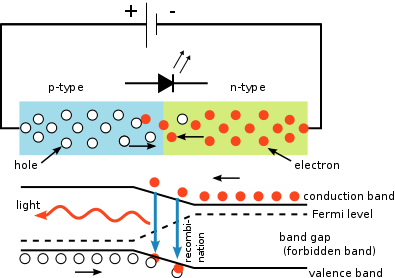
\includegraphics[height=6cm]{irodalom_res/led_working_principle.png}
    %     \caption{LED működési elve - angolul} %cite{}
    % \end{figure}
    
    Egy pár előnye a LED-es világításoknak:
        \subsubsection{Energiatakarékosság} %https://www.energy.gov/energysaver/save-electricity-and-fuel/lighting-choices-save-you-money/led-lighting
            A LED-es izzók legalább 75\%-al kevesebb energiát használnak és 25x hosszabb ideig bírják, mint a hagyományos izzólámpák. A LED-es izzók elterjedése lenne az egyik legnagyobb hatással az energiatakarékosságra. Az USA-ban például ezzel 2027-ig 348 $TWh$ elektromos munkát (egy éves teljesítménye 44, egyenként 100 Megawattos erőműnek) spórolhatnánk meg, ahhoz képpest ha nem használnánk egyátalán LED-es izzókat, ami több mint 30 milliárd dollár lenne.
            
            A hagyományos izzók teljes teljesítményének 90\%-ából hő termelődik, ami azt jelenti hogy csak 10\%-a fordítódik fénykibocsátásra. A LED-ek esetében alig termelődik hő.
        \subsubsection{Jó színvisszaadás}
            A színvisszaadási index, röviden 'CRI' (Color Rendering Index), a fényforrás azon képességét méri, hogy különféle tárgyakat megvilágítva vele, mennyire képes azok színét visszaadni. %https://hu.wikipedia.org/wiki/Sz%C3%ADnvisszaad%C3%A1s
             \begin{figure}[h!] %https://www.eledlights.com/blog/post/color-temperature-color-rendering-index-what-the-numbers-tell-you/
                \centering
                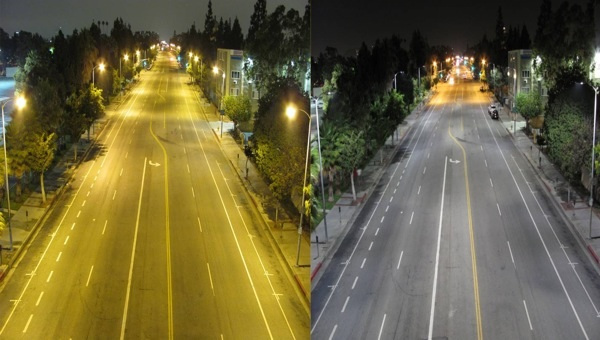
\includegraphics[height=6cm]{irodalom_res/cri_los_angeles.jpg}
                \caption{Utcai megvilágítás kisnyomású nátriumlámpával és LED-del} %cite{}
             \end{figure}
             
        \subsubsection{Környezetbarát}
            A higanylámpával és a fénycsővel ellentétben, a LED-es megoldások nem tartalmaznak higanyt.
        \subsubsection{Széles működési tartomány}
            A LED-k jól hidegben és melegben is egyaránt jól funkcionálnak, működésükhöz esetekben nagyon kis feszültségek is elegendőek, ezáltal alkalmas kültéri megvilágításokra is.
    
    \subsection{Forgalomban lévő eszközök áttekintése}
        Manapság rengeteg gyártó kínál okos világítás rendszereket. %, amelyek közül szeretnék bemutatni egy párat, illetve hogy miért érdemes alkalmazni őket. 
        Az okos égők nem csak egy átlagos LED lámpák, amiket a foglalatba lehet tekerni. Okkal hívják őket okos izzóknak. Vezeték nélkül csatlakoztathatók mobiltelefonjainkhoz, Smart Home rendszerünkhöz (Amazon Echo, Google Home), ezzel korlátlan lehetőséget kreálva. 
        
        Szinte minden ilyen izzónak lehet állítani a fényerősségét, anélkül hogy bármiféle fényerősségszabályzó kapcsolót kéne a falba szerelni. Bárhonnan vezérlehetőek, illetve be- és kikapcsolási rutinok állíthatóak be rajtuk. Ez például egy nagyszerű biztonsági funkció, mert mikor nyaralni vagyunk, akkor annak a látszatát kelti, mintha otthon lennénk. A ház elhagyása után a véletlen felkapcsolva maradt izzókat le lehet kapcsolni, nem pazarolva ezzel az elektromos áramot. A legtöbb ilyen okos lámpának a színét is lehet állítani, ezáltal a meleg- és hidegérzetünket befolyásolhatjuk. Hangulatunk nak megfelelően is behangolhatujuk, például pirosas színre állítva romantikázás esetén. A piacon zene lejátszására képes égők is elérhetők, bár ezek nem fogják a házimozirendszerünket helyettesíteni. 
        
        %https://www.cnet.com/how-to/why-your-next-light-bulb-should-be-a-smart-bulb/
        %https://www.pcmag.com/article2/0,2817,2483488,00.asp
        %pro con
        %https://www.the-ambient.com/reviews/the-best-smart-lights-bulbs-platforms-209
            
        \subsubsection{Philips HUE} %https://www2.meethue.com/en-us
            Az egyik legnagyobb háztartás- és  szórakoztató elektronikai eszköz gyártó cég is kínál okos világítás rendszereket. Talán az övéjük a legtöbb funkcióval rendelkező rendszer. Kinti, benti megoldásokat is kínálnak, zenére változó világítást és rengeteg hanggal vezérelhető opciót valósítottak meg. A telepített eszközöket, égőket egy központi egység, úgynevezett hub vezérli, illetve enélkül működőképtelen a rendszer. A Philips-hez hűen megbízhatók az esszközök, viszon cserébe elég borsos árat kell fizetni. 
            
            \begin{figure}[h!] %https://www2.meethue.com/en-us/philips-hue-benefits
                                %https://www2.meethue.com/en-us/p/hue-white-and-color-ambiance-starter-kit-e26/046677530228
                \centering
                    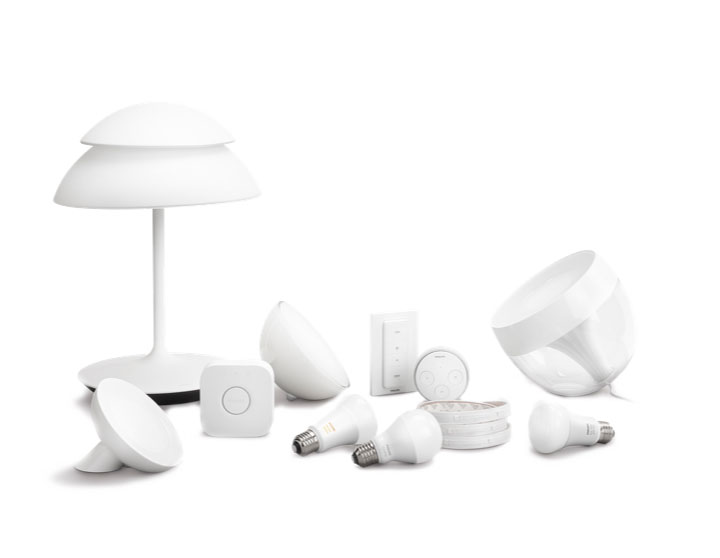
\includegraphics[height=6cm]{irodalom_res/philips_hue_termekek}
                    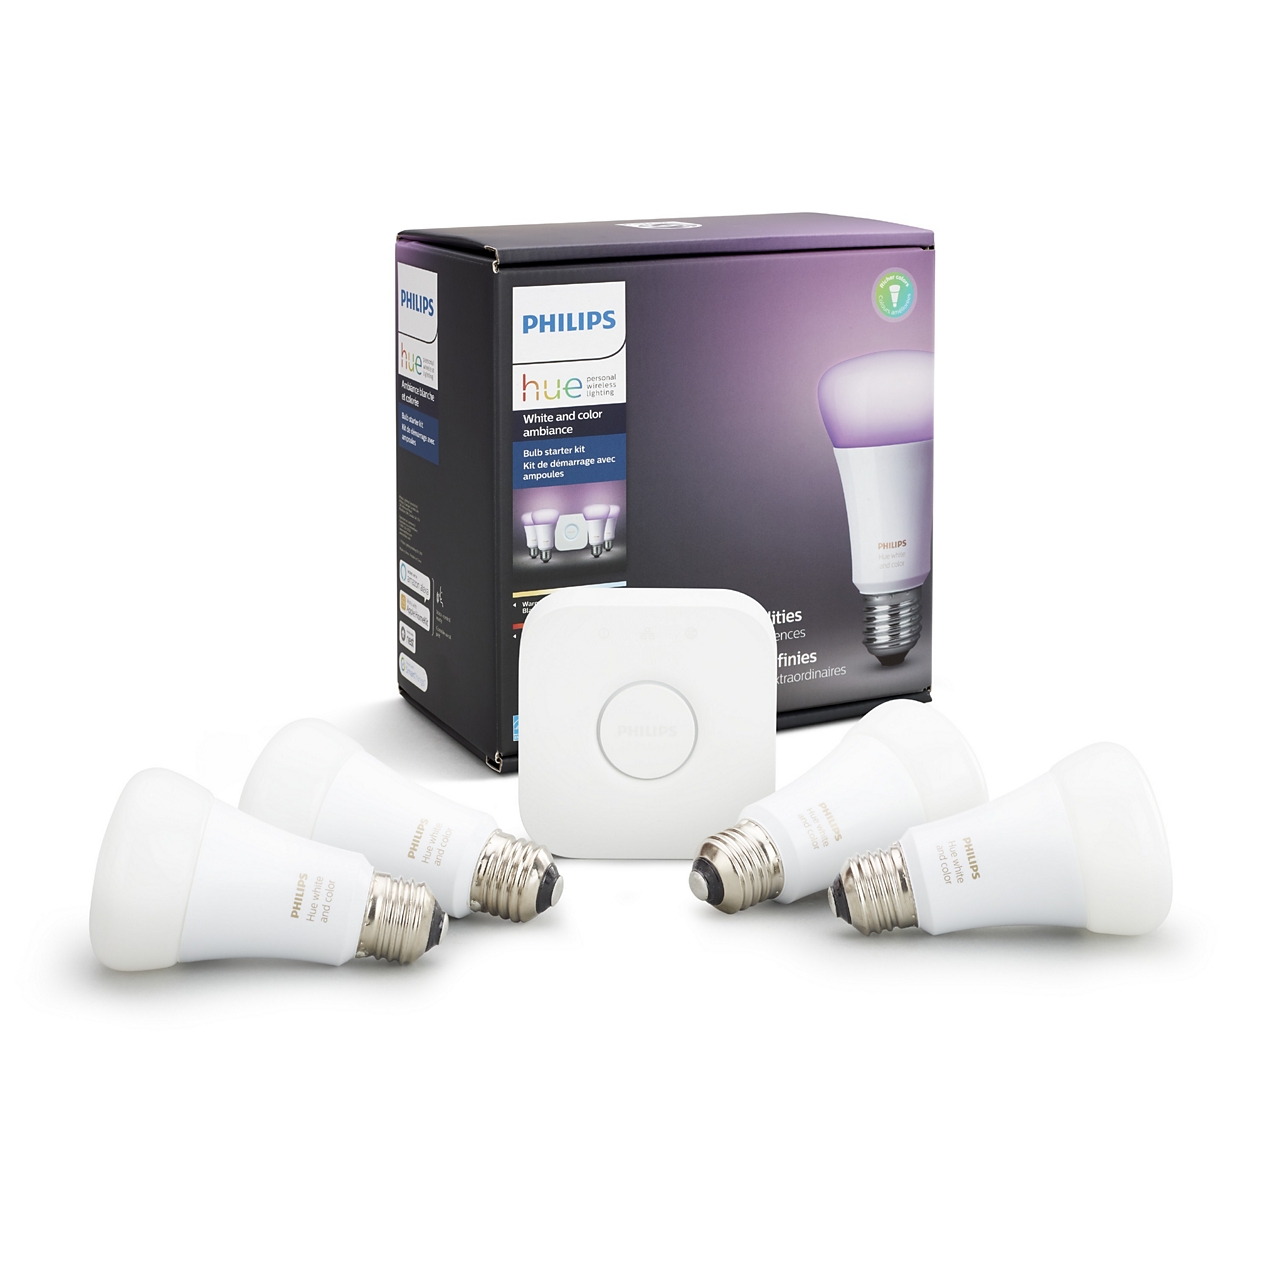
\includegraphics[height=6cm]{irodalom_res/philips_hue_termekek_2}
                \caption{Philips HUE eszközök}
                \label{fig:philips_hue}
             \end{figure}
            
            
        \subsubsection{LIFX}
            A LIFX egy okos világításra specializálódott cég. A Philips HUE termékektől annyiban különbözik, hogy ezek számára nem kell egy központi vezérlőegység, hanem képesek külön-külön működni. Egyedül a a LED szalag és csempe termékükhöz kell külön vezérlőegység. Ez a termékcsalád is vezérelhető hanggal, támogatott továbbá a Google Aszisztenst, az Apple HomeKit-et, az Amazon Alexa-t és a Logitech Harmony rendszereket is. Árát tekintve hasonló kategóriába esik a Philips termékekkel. 
            
            \begin{figure}[h!] %https://www.lifx.com/products/lifx-br30-e26?variant=15387557396554
                                %https://www.lifx.com/products/lifx-tile
                \centering
                    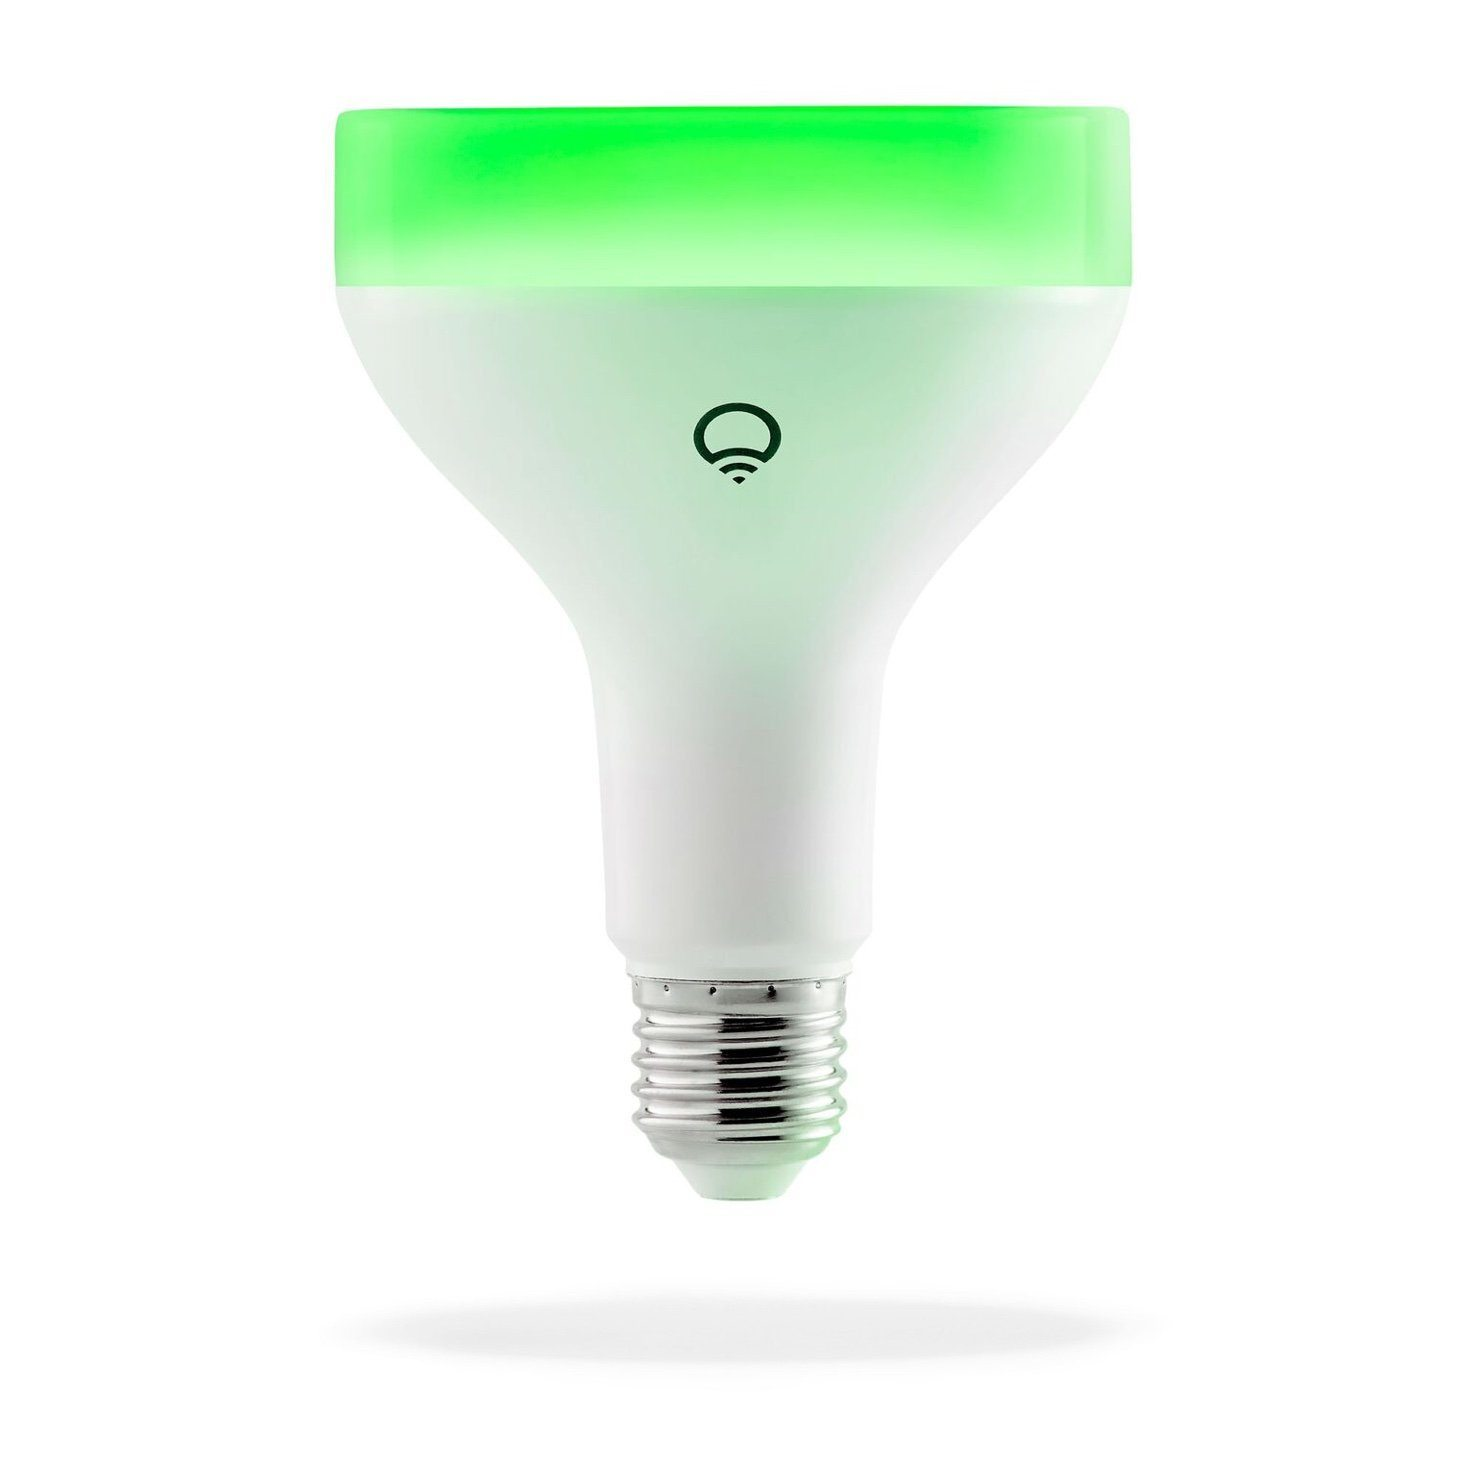
\includegraphics[height=6cm]{irodalom_res/LIFX_bulb}
                    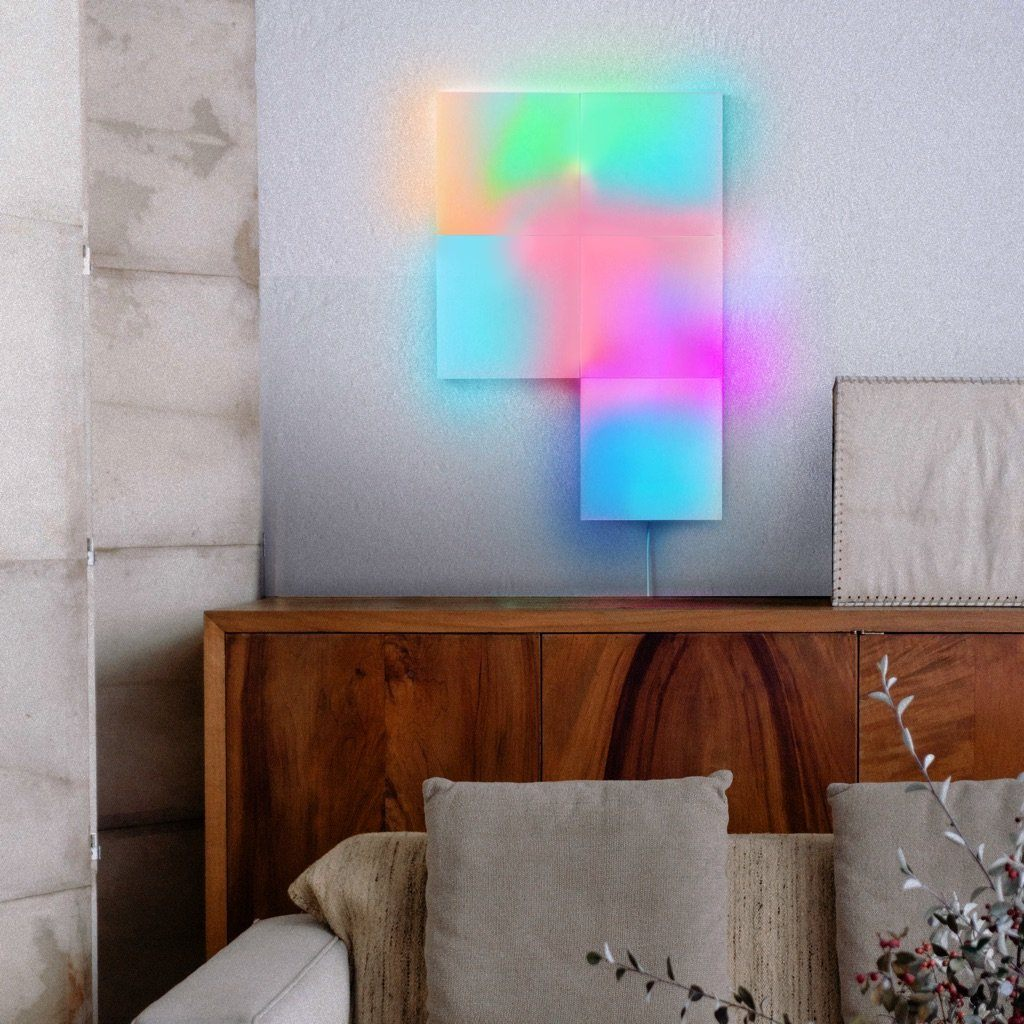
\includegraphics[height=6cm]{irodalom_res/LIFX_tile}
                    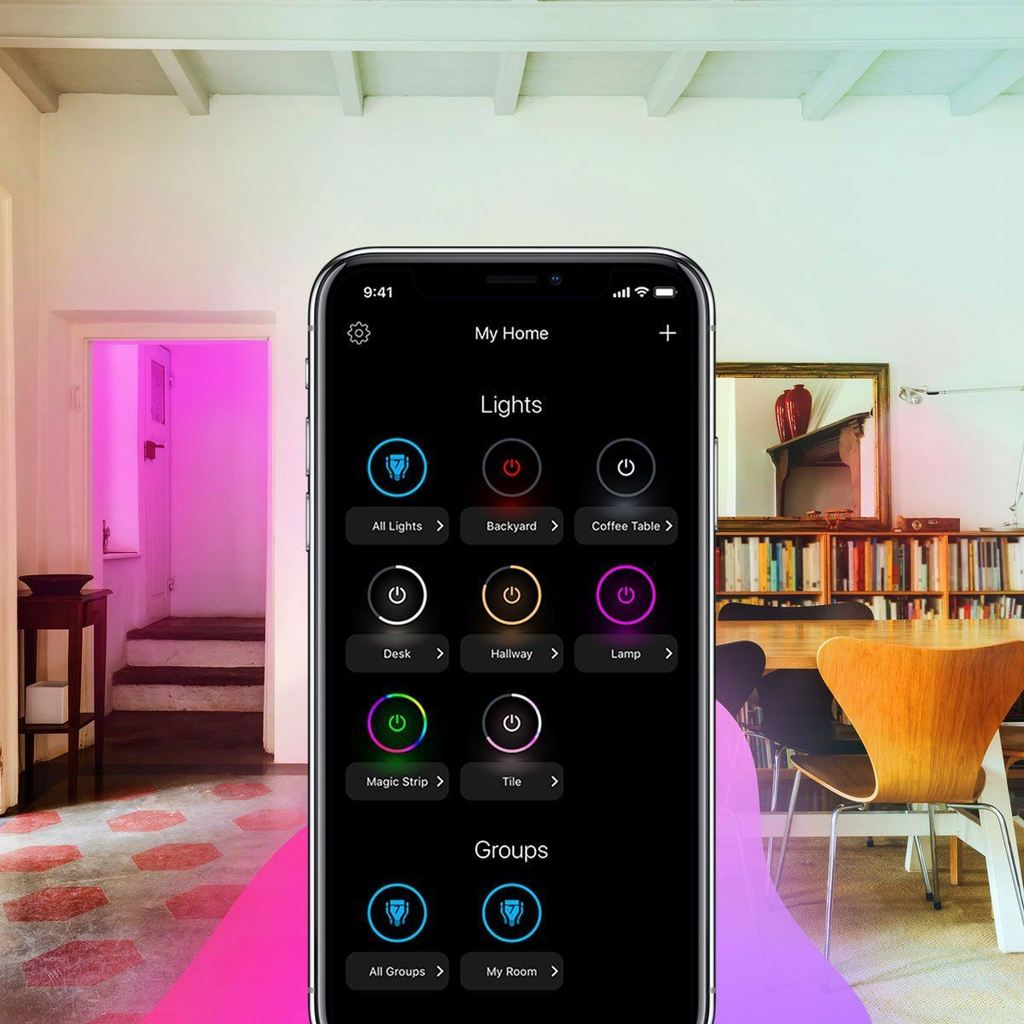
\includegraphics[height=6cm]{irodalom_res/LIFX_app1}
                    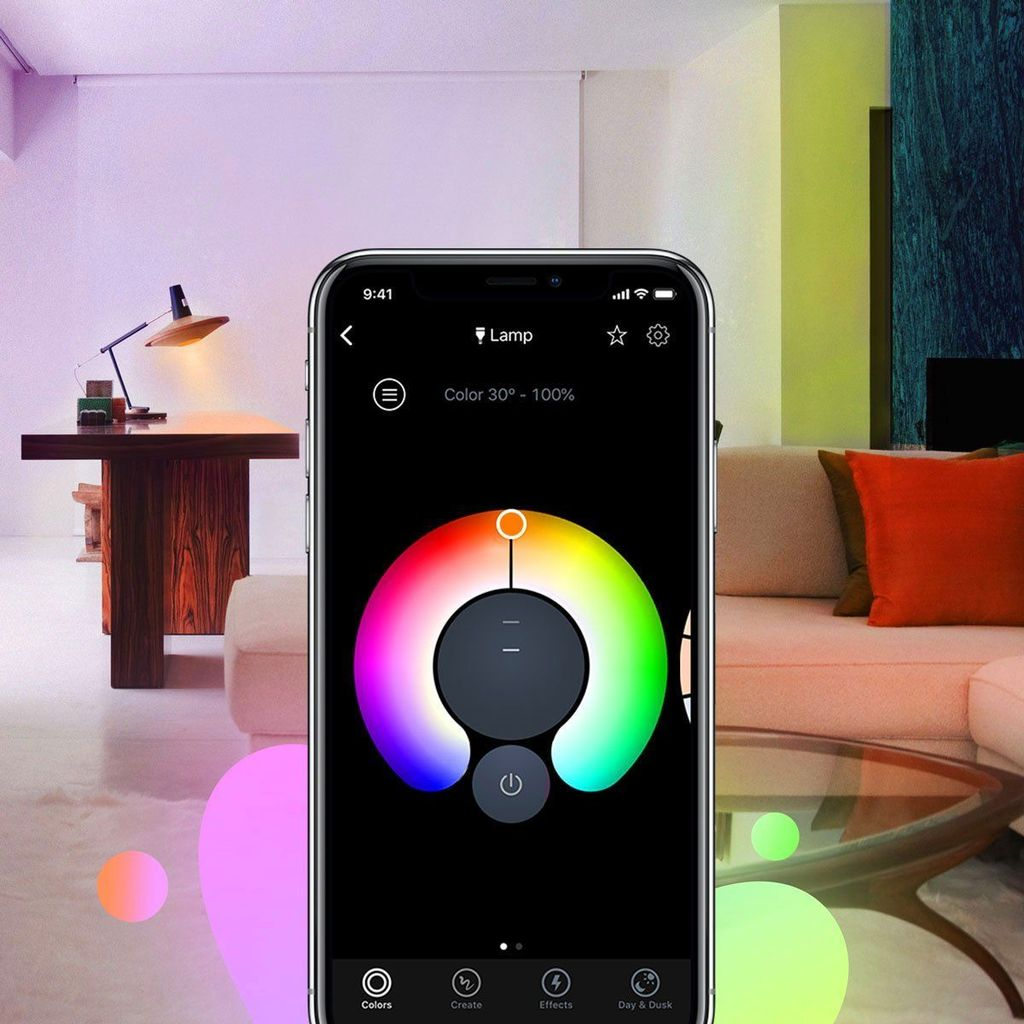
\includegraphics[height=6cm]{irodalom_res/LIFX_app2}
                \caption{LIFX termékek}
                \label{fig:lifx}
             \end{figure}
        
        \subsubsection{TP-Link okosizzó}%https://www.amazon.de/TP-Link-Gl%C3%BChbirne-funktioniert-warmwei%C3%9F-erforderlich/dp/B01N3634DR/ref=sr_1_9?ie=UTF8&qid=1542973740&sr=8-9&keywords=SMART%2BLIGHT&th=1
            A kedvező árú, vezeték nélküli hálózati eszközökről ismert TP-Link is forgalmaz okos izzókat, illetve egyéb okos otthon megoldásokat. Az ár ez esetben is kedvező, habár a vevői visszajelzések nem olyan jók mint az előző két termék esetében. A hangvezérlés Amazon Alexa-val és Google Aszisztenssel itt is támogatott.
            
            \begin{figure}[h!] 
                \centering
                    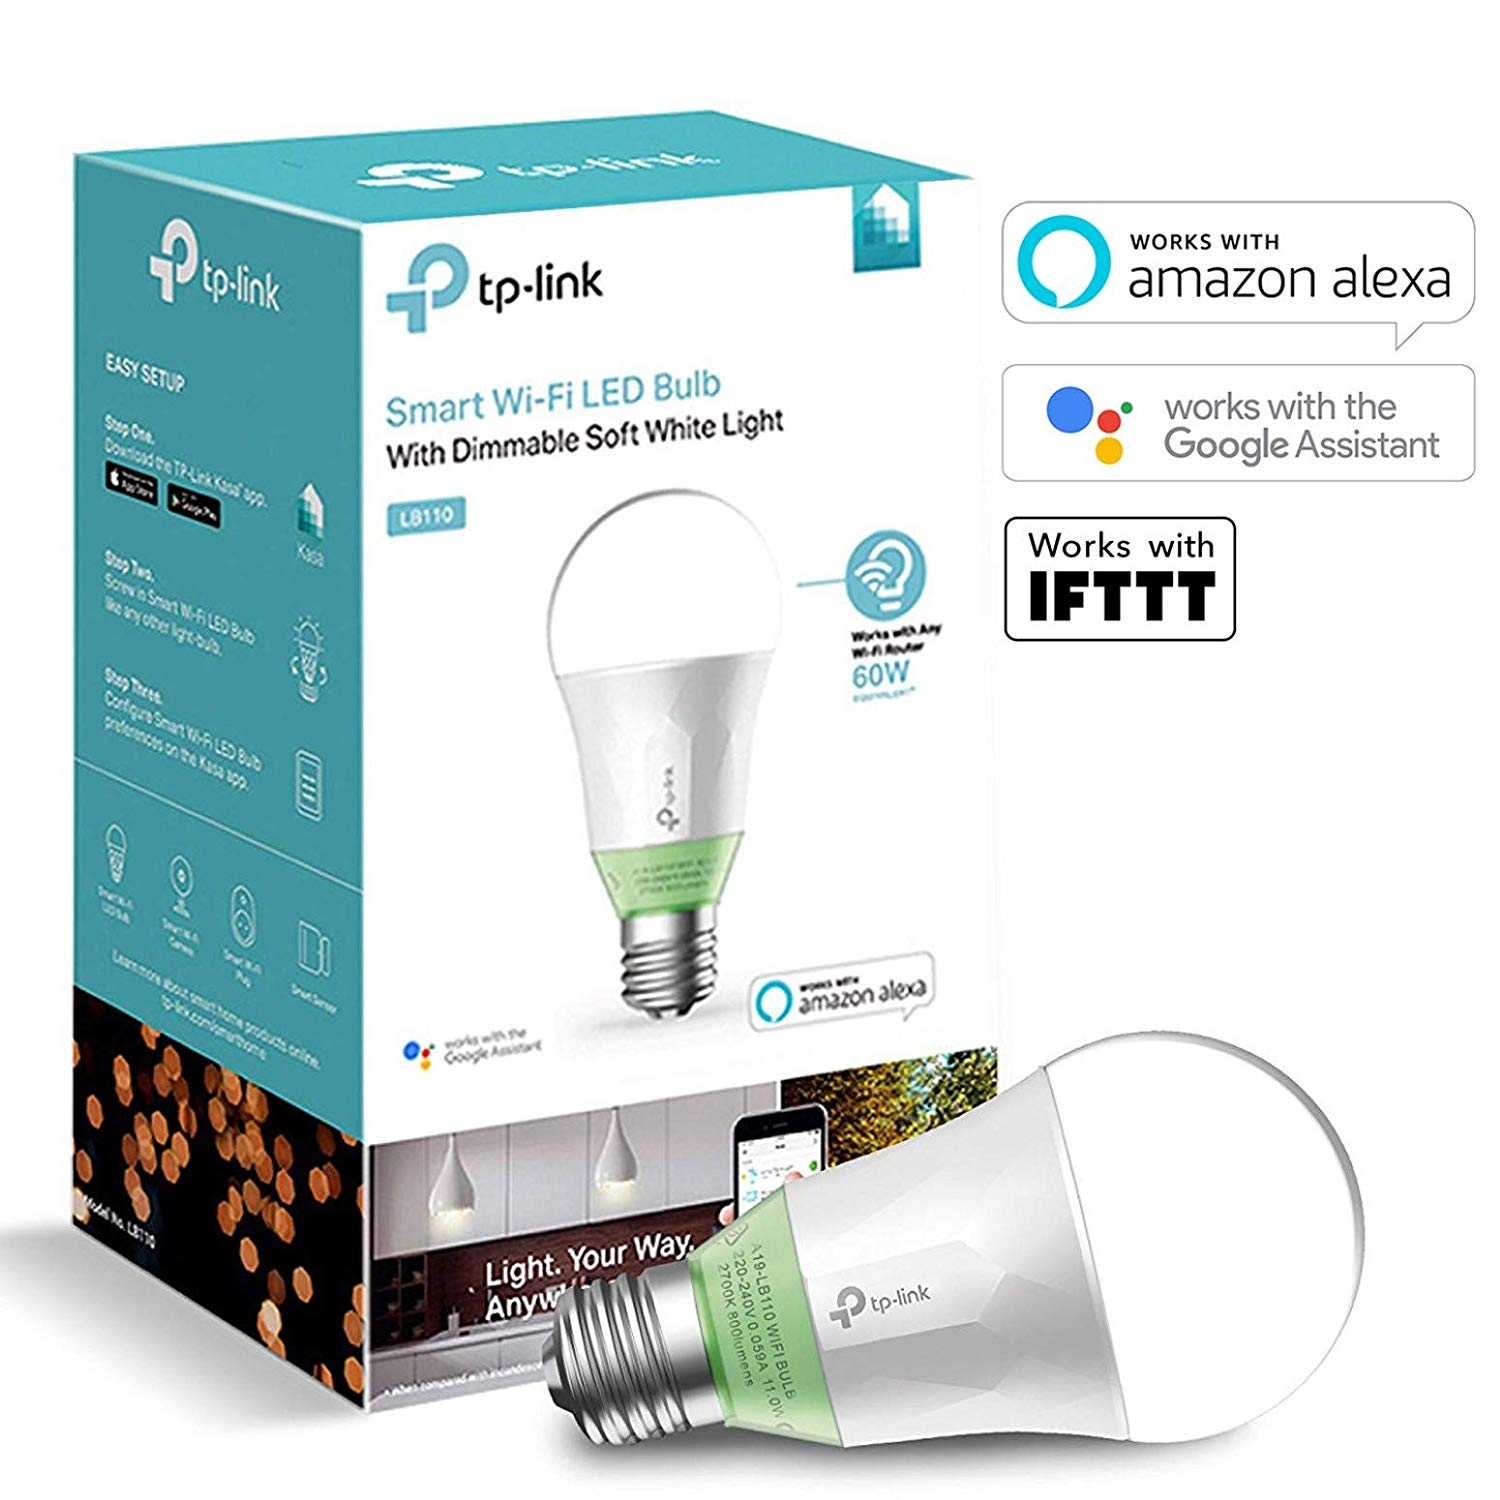
\includegraphics[height=6cm]{irodalom_res/tplink_bulb}
                \caption{TP-Link okosizzó}
                \label{fig:tplink_bulb}
             \end{figure}
        
        \subsubsection{Általásnos vezérelhető LED szalag} %https://www.ebay.com/itm/0-5M-5M-5050-RGB-LED-Strip-Waterproof-USB-LED-Light-Strips-Flexible-Tape-DC-5V/263038757504?hash=item3d3e54ea80:m:m8cgVDTTWdemEaRY1oMGGDg:rk:1:pf:0
            Talán a legolcsóbb LED-es világítás az Ebay-en, Amazon-on, Aliexpress-en, és hasonlókon rendelhető LED sorok. Ezeket többnyire áramforrással és egy egyszerűbb infrás távirányítóval működtethető vezérlőegységgel adják. Általában csak 1 szín állítható be az egész szalagon, ellentétben a címezhető LED szalakkal. 
            
            \begin{figure}[h!] 
                \centering
                    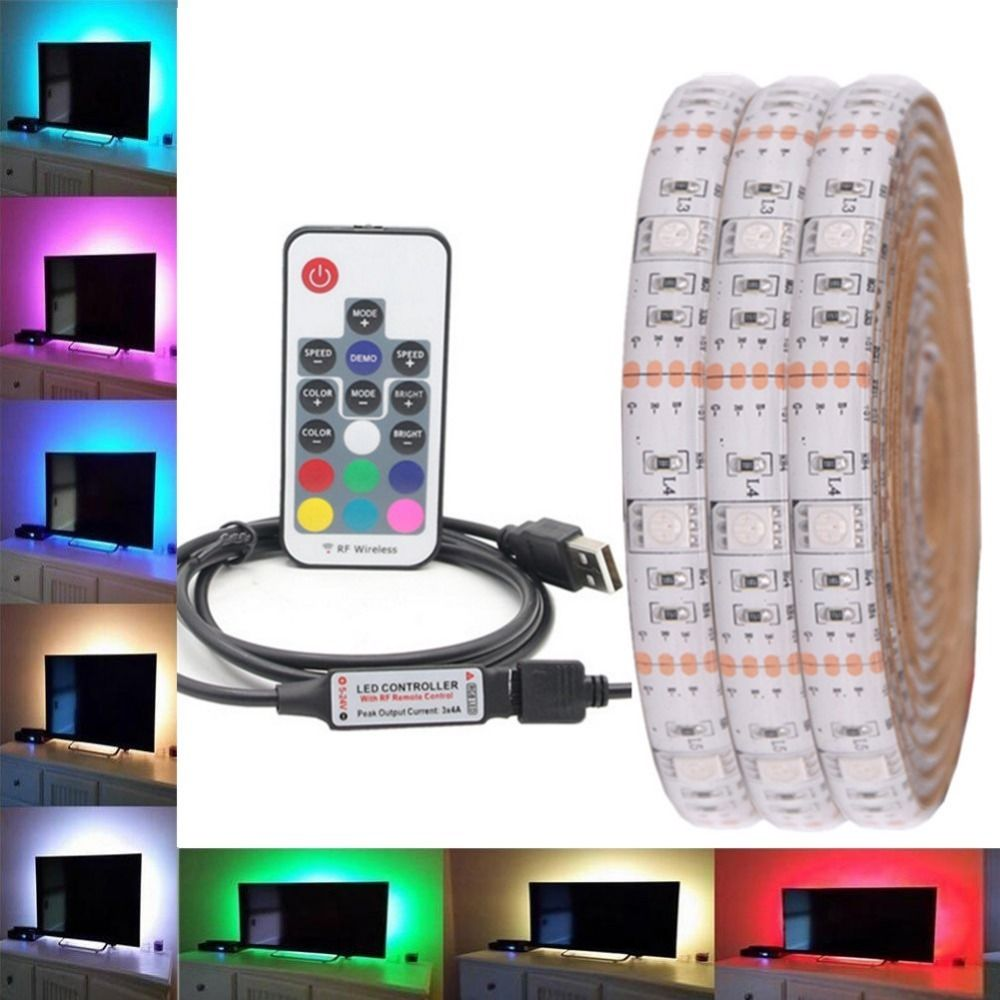
\includegraphics[height=6 cm]{irodalom_res/std_ledstrip}
                \caption{TP-Link okosizzó}
                \label{fig:std_ledstrip}
             \end{figure}
        
\newpage

\end{document}

